\documentclass[conference]{IEEEtran}
\IEEEoverridecommandlockouts
% The preceding line is only needed to identify funding in the first footnote. If that is unneeded, please comment it out.

\usepackage{cite}
\usepackage{amsmath,amssymb,amsfonts}
\usepackage{algorithmic}
\usepackage{graphicx}
\usepackage{textcomp}
\usepackage{xcolor}
\def\BibTeX{{\rm B\kern-.05em{\sc i\kern-.025em b}\kern-.08em
    T\kern-.1667em\lower.7ex\hbox{E}\kern-.125emX}}
    
\bibliographystyle{ieeetr}


\begin{document}

\title{MAKI A3 Concept Paper
% \thanks{Identify applicable funding agency here. If none, delete this.}
}

\author{
    \IEEEauthorblockN{Name Surname}
    \IEEEauthorblockA{
    Department of Mathematics \& Computer Science, University of Marburg, Germany\\
    \{\}@informatik.uni-marburg.de
    }
}

\maketitle

\begin{abstract}
% In this paper we present e study of mechanism migration and malleable transitions. 
% These two novel approaches open up transitions dedicated for non-transitionable communication systems. 
% First, potential mechanisms suitable for migration are identified, e.g., by methods of static and dynamic software analysis. 
% Methods for the migration of mechanisms are elaborated and selected mechanism migrations are investigated. 
% Specifically, suitable methods for the functional extension of non-transition-capable communication systems by new mechanisms will be explored, such as methods for modification (e.g., binary patching, library preloading, code injection) as well as preemption and redirection (e.g., proxies, splitting of data streams and/or packets). 
% Inherently extensible mechanisms are designed to ensure forward compatibility.
% Deformable transitions are realized exemplarily to gain knowledge about their applicability in real communication systems. 
% From this, recommendations for action and software design patterns for the creation of deformable transitions are derived. 
% Subsequently, the concepts of mechanism migration and deformable transitions are used in combination to realize system-wide cooperative transitions. 
% For this purpose, new mechanisms are introduced into per se non-transition-capable communication systems, which can be deployed by means of automatically adapted deformable transitions under the decision bases given by the target systems. 
% The obtained results are evaluated to demonstrate practical applicability. 
% A systematic evaluation of the performance of selected mechanism migrations and deformable transitions is performed under realistic conditions in the MAKI SDWN testbed (e.g., for web services, applications, smartphones, firmware).

\end{abstract}

\begin{IEEEkeywords}
\input{0_keywords}
\end{IEEEkeywords}

\section{Introduction}
\label{sec:intro}

In our daily life, many devices are used that are based on communication. 
This can be the smartphone, the smart light bulb or the car radio and many other. 
However, computers are not only increasingly used in private life, but also in all conceivable professional areas, for example in industry, computer-supported applications have become indispensable.  
This increased use and the long application of these systems raises the question of how the systems can be supplied with updates over time. 
With open source applications and open source operating systems this may work for experienced users, but for proprietary applications, components or systems this is only possible through the manufacturers.
Especially in the industry where the tasks only computer supported are fulfilled, many devices exist that have this dependence on manufacturers. 
But also in the other mentioned areas proprietary software, components and systems dominate the market.
As long as the manufacturer is willing and able to provide the systems with updates, there is the possibility for the hardware and software components to continue to be supplied with innovations, but if not, then the systems are frozen at this level of functionality. 
Thus, the scope of functionality depends solely on the will of the manufacturer.
Also, new challenges, for example in security, but also in the introduction of new technologies, often lead to the fact that new mechanism is not transferred to all hardware and software components. 
This quickly leads to these systems becoming legacy more quickly than would be necessary. 
By a mechanism, we refer to the concrete implementation of a functional unit that is used by the system to achieve its task. 

In particular, network systems and applications have many protocols that are not proprietary and should be more interchangeable and extensible by design. 
But the protocols used in network systems today have been standardised over a long period of time and implemented in operating systems and devices by the manufacturer.
Much of the internet traffic is based on the TCP protocol \cite{A3:john2007analysis}, which is standardised by the IETF and extended with new parts as needed. 
However, integrating new functionality into existing protocols is very time-consuming and subject to a lengthy process \cite{A3:de2019pluginizing}. 
For example, an approach has been presented in the literature that adds network coding to TCP \cite{A3:sundararajan2011network}. 
These changes are only applicable if the implementation is widely used and both sender and receiver have this extension. 
Another way would be to publish a new protocol with the new functionality instead of extend a existing protocol, but the problem remains the same. 
This creates a fundamental problem: vendor who switch to a new standard or extensions early on have hardly any advantages of their own at the beginning, but without advantages of their own, hardly any vendor will switch.
This means that it takes longer to achieve a certain spread in the market, as a certain critical mass of users must be exceeded. 

But communication protocols are only one level on which this problem occurs, as well as special parts of communication protocols like congestion control or even whole network concepts like DTN or even transmission technologies. 
All these categories have the problem that first enough systems have to be accessible for the functionality to take advantage of the usage. 
This is also true for security mechanisms that should be used for security reasons but are not available in legacy or unmodifiable systems. 
Here, the \mm can contribute to the security of systems by making these security mechanisms available.

In order to achieve the transition capability of networked systems in practice, transitions must therefore be usable on as many devices as possible.
To maximize the benefit for early adopters a method to get new functionality to legacy devices called  \mm seems to be promising.
On the one hand a \mm on the operating-system-level could be a good way to break the innovation blocking point of gaining nearly no benefits for the vendor, by intercepting communication and integrating new functionality to legacy apps and supporting new functionality os wide.
On the other hand the network itself could wrap non-changeable legacy devices to virtually bring new functionality to this devices to support a wide range of them and enable an easy way of bringing new technology much faster to legacy devices and spread new technology. 
In many areas of industry and other businesses, systems such as machines or sensor nodes are in use for many years and are not constantly renewed, especially since this would not be monetarily representable.
In these areas it is essential that new functionality are also made available to these systems.
To address this problem, among others, we introduce \mm. 

% NAT als related Work / als Interceptor
% 6in4 / 4in6
% Wine
% Interceptor Pattern aus Softwaretechnik als Inspiration
% https://patents.google.com/patent/WO2003047205A1/en20
% https://link.springer.com/chapter/10.1007/978-3-030-73885-3_14

% Vergangenheitsperspektive mehr rein bringen
% Die Vergangenheit hat uns nette Dinge gebracht
% NAT 
% Wine 

0Our contributions are:

\begin{itemize}
 \item a
 \item b 
 \item c
\end{itemize}

The paper is organized as follows. 
\section{Related Work}




\paragraph{Inherent extensibility of protocols}
There are various approaches to creating inherent extensibility of protocols.
Foundations for making network protocols extensible and updatable lie in the active networks research branch \cite{A3:tennenhouse1996towards, A3:tennenhouse1997survey}.
ANTS \cite{A3:wetherall1998ants} provides a system architecture that enables new protocols to be deployed on routers as well as terminals through platform-independent code.
Furthermore, a mechanism was presented in the literature that allows new transport protocols to be deployed easily and quickly \cite{A3:patel2003upgrading}. The protocols are exchanged between two communication partners, selected at the beginning of a connection and executed in the kernel.
An additional obstacle in the dissemination of new protocols lies in their use by applications. 
For example, Pathak et al. \cite{A3:pathak2015modnet} present a system that provides applications with additional TCP interfaces and makes TCP adaptable in a fine-grained way, but has hardly been used by applications so far.
With software-defined networks \cite{A3:mckeown2008openflow} and the network programming language P4 \cite{A3:bosshart2014p4}, network programmability was achieved. 
In particular, in the approaches described, the network devices used by providers and service providers become extensible.
Tran et al.~\cite{A3:tran2019beyond} present a method to add functionality to TCP kernel implementation using eBPF. 
As examples, the subsequent implementation of the user timeout option, as well as the dynamic change of the TCP congestion control mechanism are investigated.
QUIC is an alternative to TCP brought forth first by Google and then by the IETF, but is intended to be advanced in a similar manner to TCP.
De Coninck et al.~\cite{A3:de2019pluginizing,A3:de2018tuning} present a method to dynamically tune QUIC on a per-connection basis through extensions. In order to make the QUIC extensions platform-independent, they are executed in a virtual machine.
The presented approaches can be used by actively adapting existing systems and then enable the extensibility of these systems.


In summary, the current state of research still lacks strategies that provide for the inherent extensibility of new protocols and mechanisms -- even for domains where continuous evolution has been shown to occur in recent years. In addition, proprietary system components make it difficult to easily exchange mechanisms on common end devices. Subproject A3 aims to introduce new mechanisms into previously non-transitionable communication systems, thus enabling long-term evolution of communication systslackems.


\paragraph{Network protocols in userspace}
Network stacks are usually implemented in the operating system kernel for efficiency reasons, and existing applications use this kernel implementation. 
To introduce new functionality, it must be implemented in the kernel and adapted to the operating systems in which this functionality is to be supported.
However, network protocols can also be implemented independently of the kernel to allow faster development rates and wider distribution. 
Alpine introduces an alternative network stack in which changes can be implemented and tested quickly \cite{A3:ely2001alpine}.
MultiStack \cite{A3:honda2014rekindling} is a userspace implementation of a network stack framework that can provide isolated network stacks for different applications and enables rapid extensibility. 
An implementation of TCP in userspace is presented by Jeong et al \cite{A3:jeong2014mtcp}.
By executing in multiple threads, it is possible to achieve orders of magnitude higher bandwidth on multi-core machines, but only after the application has been adapted to the implementation.
With NUSE, the network stack of the Linux kernel can be used and further developed as a userspace library \cite{A3:tazaki2015library}. 
Existing programs can thus use modified protocols without modifications to the program itself.
Heuschkel et al.~\cite{A3:heuschkel2016virtualstack} present VirtualStack, which allows different userspace network stacks to be used on one system. 
In these network stacks, extensions as well as new protocols can be implemented and used quickly, and applications can benefit from the protocol changes in the virtual stack without adjustments. 
Especially in cloud applications, decoupling the network stack from the operating system can lead to better adaptability~\cite{A3:niu2017network}.
ClickNF \cite{A3:gallo2018clicknf} is an extension of a software-defined router in which the lower four layers of the network stack can be exchanged in a modular way. 
Extensions of existing protocols, such as TCP, can thus be implemented quickly and easily.
In order to adapt network protocols and the network stack, a system has been presented in the literature with the help of which the network stack can be detached from virtual machines (VM) and centrally managed on the host operating system and made available to the various VMs \cite{A3:niu2019netkernel}. 
SocksDirect \cite{A3:li2019socksdirect} offers the possibility for efficient socket-based communication via local networks. 
Here, a socket system was developed that is completely compatible with Linux sockets and can thus be used for them. 
This requires remote direct memory access between the communication partners in each case. 
The network stack of the operating system is replaced by its own user space implementation without having to adapt the applications. 
Furthermore, a method has been presented in the literature with which energy can be saved on smartphones by shifting parts of the processing of the network stack from the terminals to wireless base stations.
This can save cycles of CPU calculations and thus energy \cite{A3:zhu2016trimming}. 

In summary, it can be stated that despite a high number of related approaches for processing network protocols in user space, the corresponding solutions have not made broad inroads into existing communication systems. There, optimised kernel implementations of the protocols continue to dominate, which are difficult to modify adaptively. Sub-project A3 aims to demonstrate the feasibility of system modifications beyond the user space in principle and to do this, work with pre-positioning of functions and modifications of system components at runtime.



\paragraph{Software-defined wireless networks and modification of wireless communication in existing terminals}
The paradigm of software-defined radio (SDR) promises the highest flexibility in the modification of wireless communication, but to date it is predominantly limited to development platforms and is virtually unheard of in current end devices. Comparably, the approach of Cognitive Radio (CR) considers extensive reconfiguration possibilities of wireless communication with the focus on flexible spectrum use, but also requires specialised end devices. The complete functionality of SDR and CR on terminal systems would be a desirable building block for future, widely programmable communication systems. Today's reality, however, shows that commercially available terminals do not provide for corresponding modification possibilities. 

In recent years, more work on software-defined networks \cite{A3:Kreutz:2015, A3:Monsanto2013} has also been conceived beyond the programmability of the core wired network and extended to wireless communication systems \cite{A3:Bernados:WirelessCommunication, A3:Jagadeesan:2014}. Application-driven SDN-based approaches such as PANE (Participatory Networking) \cite{A3:Ferguson2013}, which served as a model for A3's work in Phase 2, assume that the end devices are completely modifiable. Qadir et al. \cite{A3:Qadir2014} give an overview of programmable wireless networks. Solutions related to subproject A3 in this area include OpenRadio (for configuring various wireless parameters) and OpenRF (for advanced MIMO signal processing with WLAN cards), in which a modification of existing terminal components was made for specialised tasks.
In Phase 2 of MAKI, corresponding work was generalised \cite{A3:ScWeHo2018, A3:GrScLiHo2019, A3:ScLiGrHo2018,A3:MaClScHo2019}, enabling programmability of wireless terminals at the lower layers.

In summary, there is so far only isolated work in wireless communication systems that -- starting from commercially available terminals -- allows a far-reaching modification of the lower network layers. Subproject A3 plans to continue the work started in Phase 2 and to enable far-reaching programmability of the lower layers in terminals as well. This will make it possible to open up non-transition-capable terminals for transitions and thus, for example, to make them capable of meeting mission-critical requirements. 



In Phase 3 of A3, the achievements of the previous phases are taken up.
Work from the areas of data-driven acquisition and adaptation of network properties, as well as participatory decision-making, will be used to construct deformable transitions. 
Nexmon and InternalBlue enabled firmware modifications for wireless network communications, laying a foundation for mechanism migration in firmware.
Inherently extensible protocols as well as user-level networking stacks represent approaches outside of MAKI and are preliminary work that will be used to achieve the goals of Phase 3. 
Taking into account the work presented, a novel methodology is created in A3 to achieve non-transitionable communication systems transition capability using mechanism migration and to deploy malleable transitions under the given framework.

\section{Design}
\label{sec:design}

Networked systems as used today consist of many hardware and software components that are connected to each other to achieve their intended task.
Hosts in a network use gateways to communicate with hosts in other networks, user space applications use system calls to interact with the operating system and hardware components use interfaces to achieve interaction between each other, such as PCI.
However, many of the components can not be updated or upgraded, either due to their proprietary nature or due to lengthy standardization and deployment processes.
This hinders the development of novel applications or improvements of existing systems.
However, developers and engineers already found a way to overcome this problem, by utilizing the environment of such systems and force it behave as desired.

\subsection{Unobtrusive Mechanism Migration by Example}
To illustrate this idea, two examples will be given.

\subsubsection{Network Address Translation}
The Internet Protocol version 4 (IPv4) was designed in the late 1970s and deployed throughout the 1980s.
At that time, the number of participating hosts in the Internet was rather low with less than 1000 and the designers of IPv4 did not anticipate, that the number of hosts in the Internet would increase dramatically as it did especially since the 2000s.
Thus, they chose a 32 Bit field for addressing, allowing only roughly 4.3 billion hosts in the Internet.
With over 5.5 billion devices~\cite{eriscsson2021report}, there are even more smartphones already available globally, not to mention servers, wearables, embedded systems and the entire IoT area.
This development raised the need for solutions.
Althouth there is a newer version of the IP, IPv6 allowing $2^128$ ho

Das erste Beispiel: NAT
Problem, das NAT lösen soll: IPv4 Adressen gibt es zu wenige. Das Ausrollen neuer, besseren Standards dauern jedoch lange, müssen parallel betrieben werden
Sytem: Host, der über das Internet kommunizieren möchte
Environment: Netzwerkzugang
Interceptor: Softwarekomponente auf dem Gateway, der das masquerading anbietet.
Alter mechansimus: routing auf dem Gateway
Neuer Mechanismus: routing wird druch hinzugefügtes masquerading ersetzt
Hinweis: dieses beispiel sollte etwas ausführlicher dargestellt werden, also was wird konkret intercepted, wie findet die Übersetzung statt.

\paragraph{Example 2: WINE}
Zweites Beispiel: Wine
Problem: Ausführung von Programmen auf Betriebssystemen mit inkompatiblen Schnittstellen und Bibliotheken; eine spezifische Implementierung in eimem Anderen Betriebssytem würde das Problem nur für das spezifische System lösen, wine löst es generell durch das Interceptor patter.
System: Programm
Environment: Betriebssytem
Interceptor: Sammlung an überschriebenen Sytemaufrufen und Bibliotheken, Wine
Alter mechanismus: Nutzung der vom betriebyssytem bereitgestellten systemafurufe und bibliotheken
neue Mechanismus: Nutzung von POSIX schnittstellen über hinzugefügte systemafurufe und bibliotheken
Hinweis: auch dieses Beispiel ausführlicher Beschreiben

Die Informatik ist voll von solchen Abstraktionen, etwas <hier zwei weitere Beispiele einsetzen>.
Das ist nicht nur eine Anomalie oder Ausnahme von Funktionserweiterung.
Wie posulieren, dass dieses Vorhegen System hat, sodass wir eine Abstraktion definieren.


\subsection{System Model}
\begin{figure}
    \centering
    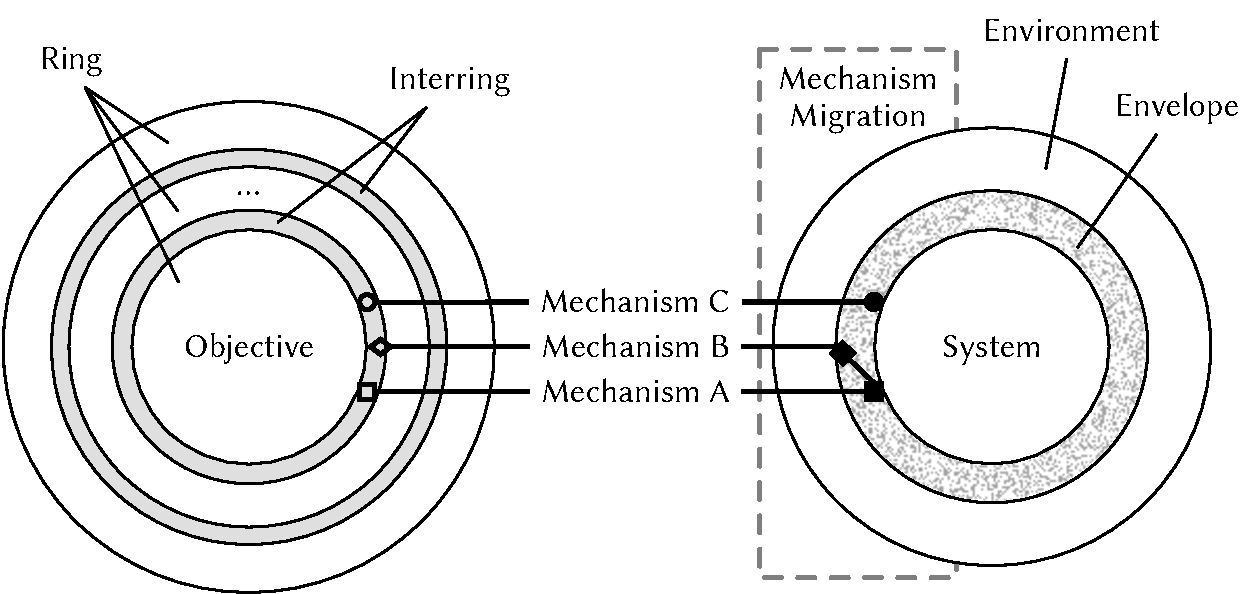
\includegraphics[width=\linewidth]{figures/MechanismMigration.pdf}
    \caption{Mechanism migration to a legacy device with transition-enabled environment}
    \label{fig:bigpicture}
\end{figure}

% Das von uns abgeleitete Modell besteht aus folgenden Komponenten:
The model derived from the above examples and further observations consists of the following components:


\paragraph{System}
At the core of the consideration lies a system that is intended to achieve a specific task.
The system cannot be changed because it is a proprietary component or depends on other external factors, such as high coordination costs for changes due to long standardization or technical hurdles.
This is necessarily so that the system can fulfill its actual task. 
For example, the host in the NAT example needs the routing functionality of the gateway to enable communication with hosts in other networks.

\paragraph{Environment}
Every system is surrounded by an environment that provides functionality for use.
The system has a dependency relationship with the environment, as the system is dependent on the functions provided.
This is necessarily so that the system can fulfill its actual task. For example, the host in the NAT example needs the routing functionality of the gateway to enable communication with hosts in other networks.

\paragraph{Mechanism}
By a mechanism, we refer to the concrete implementation of a functional unit of the environment that is used by the system to achieve its task.
% By a mechanism, we refer to ''a confined conceptual element of a (networked) system that is bound to a realization as cooperating functional units''~\cite{frommgen2016mechanism}.
Mechanisms are located at various points of hardware/software systems, for example:

\begin{itemize}
 \item Complete protocols: TCP, UDP, RTP, overlays, etc.
 \item Specific parts of protocols: congestion control, fragmentation, load balancing, replication, etc.
 \item Network concepts: infrastructure-based, ad-hoc, partially meshed, delay tolerant (DTN), etc.
 \item Network technologies: Ethernet, LTE, IEEE 802.11, Bluetooth, etc.
 \item Security mechanisms: encryption, integrity protection, authentication, etc.
 \item System components: positioning (via WLAN, GSM or GPS), sensors, etc.
 \item Operating System APIs
 \item System Bus Interfaces
\end{itemize}



\paragraph{Interceptor}
In the field of software development, the ``Interceptor architectural pattern allows services to be added transparently to a framework and triggered automatically when certain events occur''~\cite{schmidt2013pattern}.
In this programming pattern, a framework provides interfaces so that programs using this framework can transparently intervene in the flow of data at specific events.

While the goal of our interceptor is basically the same, namely to transparently intervene in the data flow and thus enable new functionalities, the perspective is reversed.
An interceptor in our definition is part of the environment and provides mechanisms to the system via known interfaces. 
In contrast to the interceptor pattern of software engineering, the interceptor is used by the system but configured by the environment so that its use is inevitable.
In order for the system to use the new mechanism, the interceptor is inserted between the system and the mechanism and changes the data flow.
The mechanism to be used can also be introduced into the environment as part of the interceptor and does not have to exist a priori. 


\paragraph{Unobtrusive}
In order not to influence or even disturb the actual task of the system, the mechanism from the interceptor must be unobtrusively replaced by the provided mechanism.
The system must not notice the change of the mechanism, on the contrary the used interfaces must suggest that the original mechanism would be in force.
Furthermore, an interceptor must be unobtrusive so that the system can continue to fulfill the functionality and not provide error cases for the termination.




































%%%%%%%% OLD %%%%%%%%%%%%%
% \begin{figure}
%     \centering
%     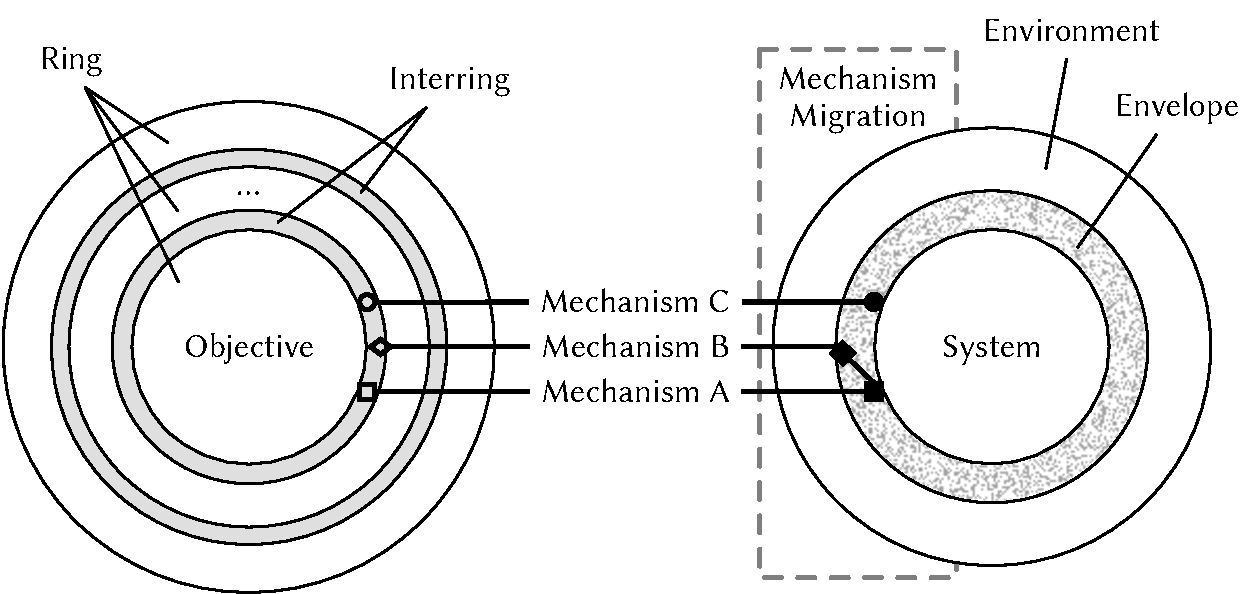
\includegraphics[width=\linewidth]{figures/MechanismMigration.pdf}
%     \caption{Mechanism migration to a legacy device with transition-enabled environment}
%     \label{fig:bigpicture}
% \end{figure}

% The concept of \emph{\mm} allows altering behavior of information and communications system (ICS) that are incapable or unwilling to modify their own operation.
% This could be due to an ICS being built upon proprietary frameworks disallowing modification of the device, manufacturers dropping support or by the unwillingness to make the effort to adapt or update the components of the ICS.
% In such cases developers or network operators are unable to modify the ICS itself.
% However, the proposed approach of \mm enables the modification of an ICS's environment to enforce the desired adaption in its behavior.
% This change can be thought of as an ''outer'' level of the communication infrastructure enveloping an ''inner'' level.

% For example, when faced with a closed application executed on a smartphone, operating system (OS) might be modified to force the applications behavior to change by modifying the OS network stack to transparently wrap connection in a VPN.
% If a whole device is unmodifiable, but the network is under control of the network operator the network can be utilized to force the device to behave in a desired way, e.g. by placing gateway-servers inside the network who can transparently alter traffic flows.
% If even the network is outside control modifying or replacing the communication partner/backend with which the device is communicating is possible.


% \subsection{Rings}
% As the above examples suggest, modern information and communications technology consists of a multitude of components like access devices (smartphones, computers, etc.) and network infrastructure (routers, back-bone network), software (e.g., OSs, middle-ware, applications), networks, network topologies, network protocols on various layers, compute facilities (cloud, edge, etc.) and so on.
% We subdivide these components into a ring structure, as shown in \Cref{fig:bigpicture}, where each \emph{ring} represents a component required for the given domain.
% The most specific component, whose functionality is to be improved by the proposed \mm, forms the center of the structure, called \emph{objective}, while other components are added as rings.
% As an example, an ICS providing a VoIP service to users, the telephony application installed on the end-users device would form the objective, as it should be modified in some way.
% This application requires the OS and its networking APIs, which forms the ring around the application, whereas the next outer ring forms the local area network.
% This categorization allows arbitrary deep rings that seem appropriate for the given domain.
% In the above example, the outer most ring would be the backend executed on a server in the cloud.
% For enabling \mm, it is important to be able to modify or alter rings around the objective, although it is not required to have control of all rings but only the ring required to achieve the desired result.


% \subsection{Interrings}
% Between adjacent rings, components require interaction.
% Such an interface can be anything from set of rules governing the actual communication, such as protocols defined on the different layers of the network-stack-model, to implicit assumptions over the inner workings of peers in a network.
% In the above example, the telephony application uses the OS's networking API to send and receive data.
% Thereon, the OS uses for example Wi-Fi or cellular connectivity to access the local area network, and so on.
% These interaction layers are called \emph{interrings} and are represented as gray layers between the rings in \Cref{fig:bigpicture}.
% Beyond the network stack on a local device itself, interrings include any functionality that allows interaction between two rings like system calls in an application-OS relation or communications between multiple nodes in a network.


% \subsection{Mechanism}
% A \emph{mechanism} is a functional part of an interring that realizes functional units to achieve the desired functionality of the objective.
% Examples of such mechanisms are manifold and span all protocol- and system-layers, as the following selection of possible mechanisms shows:

% \begin{itemize}
%  \item Complete protocols: TCP, UDP, RTP, overlays, etc.
%  \item Specific parts of protocols: congestion control, fragmentation, load balancing, replication, etc.
%  \item Network concepts: infrastructure-based, ad-hoc, partially meshed, delay tolerant (DTN), etc.
%  \item Network technologies: Ethernet, LTE, IEEE 802.11, Bluetooth, etc.
%  \item Security mechanisms: encryption, integrity protection, authentication, etc.
%  \item System components: positioning (via WLAN, GSM or GPS), sensors, etc.
% \end{itemize}

 

% \subsection{Envelope, System and Environment}
% In order to realize the proposed approach, it is necessary to migrate novel functionality to existing ICS.
% An \emph{\env} is a component containing such a new or alternative mechanism that is migrated to the interring between the last ring that is under control and the first ring that is not under control.
% For example, if the telephony application that should support vertical handovers is not modifiable but the OS, the \env containing a mechanism enabling vertical handovers could be placed in the interring between application and the OS.
% It might also be desirable to migrate an \env into an outer interring, although a ring closer to the objective might be still under control.
% All rings, including the objective, that are located within the \env are summarized as the \emph{system} and all rings outside the \env are called \emph{environment}.

 
\input{4_implementation}
\input{5_evaluation}
\section{Conclusion}
\label{sec:conclusion}

We presented \emph{\mm}, a novel approach providing a model to implement unobtrusive functional additions to or modifications of an existing networked system without touching any proprietary components.
By classifying a networked system into the \emph{system}, i.e., components containing proprietary or other not changeable parts, and the \emph{environment}, i.e., components containing modifiable parts under control, 
behavioral changes are achieved by mechanism-enhancing yet unobtrusive \emph{interceptors},
i.e., a layer that is introduced between environment and system adding or updating mechanisms.
Such an interceptor can have many forms like an updated software library, a newly deployed edge device, or an enhanced cloud service.
Interceptors must be unobtrusive to avoid disrupting or even breaking applications but still provide added or modified mechanisms to the networked systems.

We illustrate this approach by applying the findings of the model in two case studies
that show its real-world applicability.
First, we unobtrusively replace a cloud infrastructure by an edge infrastructure in a wireless sensor network.
Second, we unobtrusively add a vertical handover mechanism between Wi-Fi and LTE to a mobile end device without disconnecting TCP sessions.
Our results indicate that \mm is a compelling approach to achieve improved service quality and provide previously unavailable functionality in an unobtrusive manner.

The contributions of this paper are:
\begin{itemize}
    \item We present \mm, a model that can be used by developers to design and implement unobtrusive mechanism interceptors.
    \item We present two examples, NAT and Wine, which serve as a basis for developing the \mm model.
    \item We present an application, \ttt, where our model is applied to replace a cloud infrastructure by an edge infrastructure to unobtrusively add previously unavailable functionality in a sensor network.
    \item We present an application, where our model is applied to add an unobtrusive vertical handover mechanism between Wi-Fi and LTE and thereby improve service quality of mobile devices.
\end{itemize}

The remainder of this paper is organized as follows.
Section~\ref{sec:releted_work} presents related work.
Section~\ref{sec:design} introduces two real-world examples and the derived model for \mm.
Section~\ref{sec:treetalker} presents the first case-study, \ttt and Section~\ref{sec:wg:impl} presents the second case-study, \wgh.
Section~\ref{sec:conclusion} concludes this paper and presents future work.


\section*{Acknowledgments}
This work is funded by the Hessian State Ministry for Higher Education, Research and the Arts (HMWK) (LOEWE Natur 4.0, and LOEWE emergenCITY), the German Academic Exchange Service (DAAD) (Transformation Partnership Program; Project OLIVIA), and the German Research Foundation (DFG, Project 210487104 - Collaborative Research Center SFB 1053 MAKI).


\bibliography{main}

\end{document}
